\renewcommand{\documentname}{Annexes}

\chapter{Annexes}


\section{Definitions and abbreviations}\label{defs-abbrev}

Listed below is a glossary of definitions and abbreviations used in the document whose meaning may not be obvious.

Glossary of definitions:

\begin{itemize}
    \item \textbf{Evolutionary Computation:} method of designing a metaheuristic algorithm. It is a subtype of Population-based methods. The definitions for the common components of evolutionary computation follow \cite{luke13metaheuristics}.
        \begin{itemize}
            \item \textbf{Breeding:} the act of creating one or more children from a population of parents by combining the crossover and mutation operators.
            \item \textbf{Chromosome:} a specific type of genome consisting of a fixed-length array.
            \item \textbf{Child and parent:} both are individuals. A child being a possible modification of its parent.
            \item \textbf{Crossover:} operator that creates childs from parents by means of combining sections of the genomes of the parents.
            \item \textbf{Evaluation:} calculating the fitness of an individual.
            \item \textbf{Fitness:} quality of an individual.
            \item \textbf{Generation:} the population of a given iteration of the algorithm. The next generation is created by means of the different operations defined by said algorithm.
            \item \textbf{Genome:} the data structure that defines an individual.
            \item \textbf{Individual:} candidate solution for the problem.
            \item \textbf{Mutation:} operator that modifies the genome of an individual.
            \item \textbf{Population:} set of individuals.
            \item \textbf{Selection:} operator that elects individuals from the population based on some criteria.
        \end{itemize}
    \item \textbf{Genetic algorithm:} metaheuristic search and optimization algorithm. 
    \item \textbf{Greedy algorithm:} algorithm that builds the solution in successive steps, always trying to take the optimal solution for each step
    \item \textbf{Heuristic:} function that gives value to each path from a intermediate state to the goal state. Applied in search algorithms, heuristics are based on knowledge outside the problem definition.
    \item \textbf{Java:} general-purpose, high-level, object-oriented programming language.
    \item \textbf{Metaheuristic:} algorithm that uses randomness to find a possible optimal solution to a hard problem. They are part of the stochastic optimization field.
\end{itemize}

Glossary of abbreviations:

\begin{itemize}
    \item \textbf{CSV:} Comma-Separated Values. Refers to a text file format.
    \item \textbf{CLI:} Command Line Interface.
    \item \textbf{EA:} Evolutionary Algorithm.
    \item \textbf{EC:} Evolutionary Computation.
    \item \textbf{ES:} Evolution Strategies.
    \item \textbf{GA:} Genetic Algorithm.
    \item \textbf{LCM:} Lazy Collision Matrix (see \ref{lcm}).
    \item \textbf{LFD:} Lazy Filter Dictionary (see \ref{lfd}).
    \item \textbf{UC:} Use case. 
    \item \textbf{TXT:} Text. Refers to the text file format.
    \item \textbf{WBS:} Work Breakdown Structure.
\end{itemize}



\section{Work Breakdown Structure (WBS)}


\begin{figure}[H]
    \caption{WBS (Bigger scale)}
  \centering
  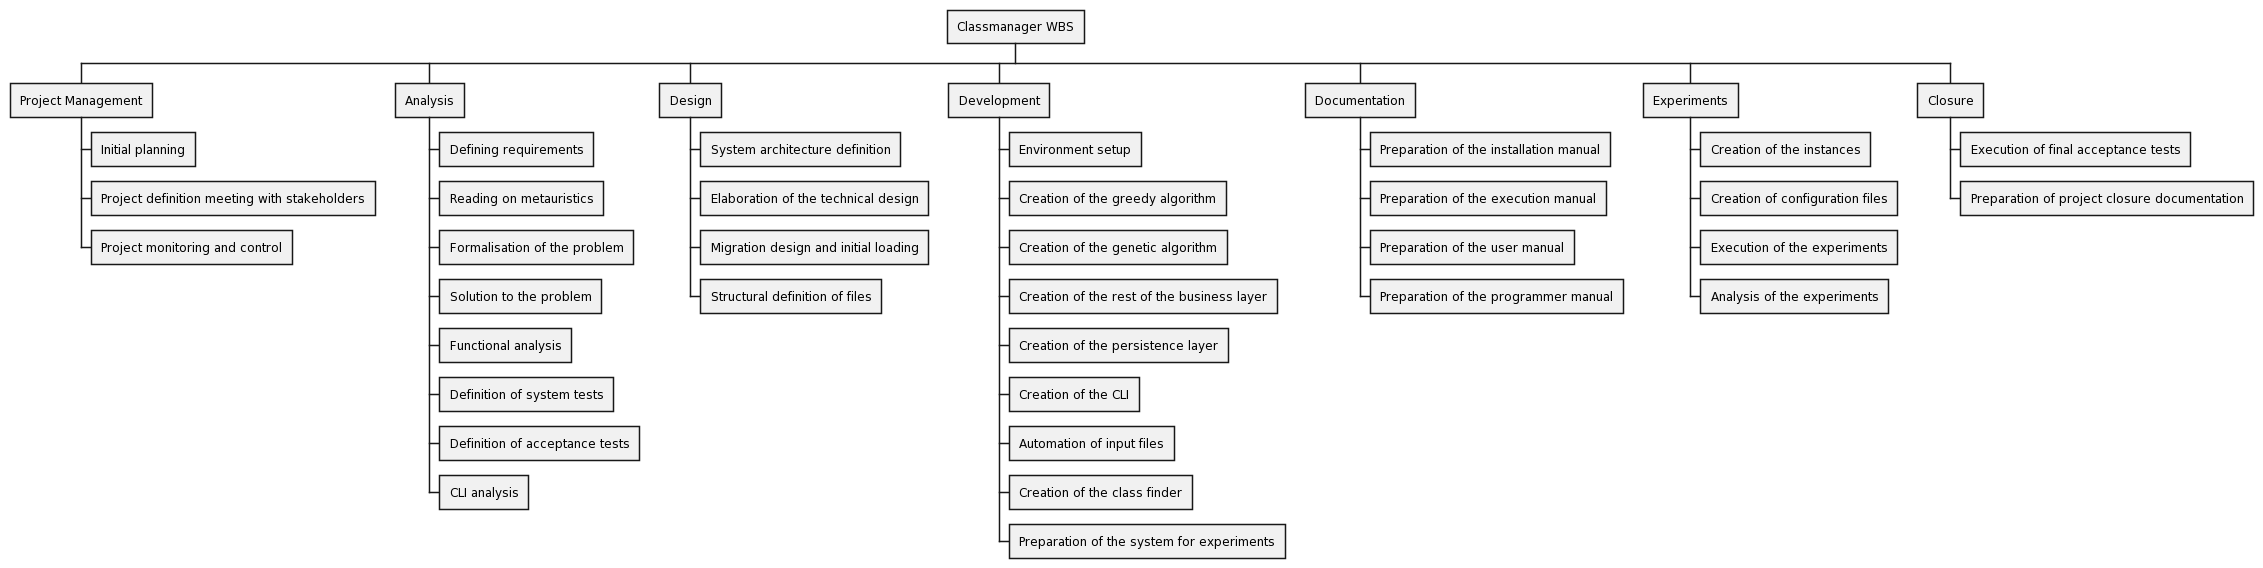
\includegraphics[scale=0.26, angle=90]{wbs.png}
\end{figure}



\section{Submission contents}

\subsection{Code}



\subsection{System and external files}\label{annex-file-format}

Compressed archive with examples of all files involved with the system. Its structure is as follows.

\begin{description}
    \item \textbf{annexfileformat/}
        \begin{description}
            \item \textbf{ucassignments/}
                \begin{description}
                    \item \textbf{config/}
                    \item \textbf{input/}
                    \item \textbf{output/}
                \end{description}
            \item \textbf{ucfreeclassrooms/}
                \begin{description}
                    \item \textbf{config/}
                    \item \textbf{input/}
                    \item \textbf{output/}
                \end{description}
            \item \textbf{ucautomation/}
                \begin{description}
                    \item \textbf{config/}
                    \item \textbf{input/}
                    \item \textbf{output/}
                \end{description}
            \item \textbf{classmanager\_log/} (LOG examples)
        \end{description}
\end{description}

